%
% Latex example file for postgrads (04/10/03)
%
% If you have questions please email me: 
% M.L.Balogh@durham.ac.uk
% or find me in room OC312.
%
% Note you can get Latex style files etc. from http://www.ctan.org


% Use emulateapj instead to make Apj format.
% YOU SHOULD REMOVE THE TABLE OF
% CONTENTS PAGE WHEN USING APJ FORMAT.
\documentclass[11pt,a4paper]{emulateapj}
\bibliographystyle{apj}


%define general packages
\usepackage{epsfig}
\usepackage{amsmath}
\usepackage{natbib}

% spanish packages
\usepackage[utf8]{inputenc}
\usepackage[spanish]{babel}
\languageshorthands{none}
\noextrasspanish
\let\layoutspanish\relax
\usepackage[spanish]{babel}
\renewcommand\shorthandsspanish{}

%internal short cuts
\def \HgA {H$\gamma_A$}
\def \gon {Gonz\'{a}lez}
\def \Hbp {H$\beta ^\prime$}
\def \warn {{\sffamily\bfseries\large WARNING, ARREGLAR:}}









\begin{document}

\submitted{Departamento Ing. en Informática, ITBA}
\title{La soga en el iPhone}
\author{Williams M. \& Aráoz M.}
\date{\today}


\begin{abstract}
El diseño de un reactor nuclear es un problema muy interesante y complicado. Simplificando el
modelo para 1 dimensión es posible predecir numéricamente el comportamiento de los neutrones
producidos por la fusión nuclear. En este trabajo se aplica un método de la potencia con una 
leve modificación para alcanzar dicho fin.
\end{abstract}

\maketitle




\section{Introduccción}
\label{sec:introduccion}
La ecuación de ondas se puede utilizar para representar diferentes objetos de la vida cotidiana. La forma más simple de representar la ecuación de ondas es la siguiente:
\begin{equation}
\label{eq:ondas}
\frac{\partial ^2 u}{\partial t^2} = c^2 \nabla ^2 u
\end{equation}
, donde $\nabla ^2$ es el laplaciano y $c$ es una constante que depende del problema. Para poder hacer uso de la ecuación (\ref{eq:ondas}) dentro de un dispositivo de cálculo se debe discretizar la ecuación con el fin de obtener una aproximación que se pueda ingresar al dispositivo. Para lograr esto primero se debe obtener una aproximación de las derivadas parciales y luego se debe discretizar estas aproximaciones. Luego de realizar esto, se obtiene el siguiente método para calcular $u(x,t)$ de forma aproximada a partir de las condiciones de borde del problema $u(0,t) = L_1$ y $u(L,t) = L_2$ teniendo en cuenta que $0 < x < L$ y de la condición inicial $u(x,0) = g(x)$:
\begin{eqnarray}
	\label{eq:metodoDeOndas}
	\left\{
		\begin{matrix}
			u_i^{n+1} = (2-2r) u_i^n + r^2 (u_{i-1}^n+u_{i+1}^n) - u_i^{n-1}\\
			u_j^0 = g(\Delta x j)\\
			u_0^n = L_1\\ 
			u_N^n = L_2\\
		\end{matrix} \right.
\end{eqnarray}
Este método se utilizó para en este trabajo para realizar una simulación del comportamiento de una soga en un iPhone. A la soga se le pueden efectuar perturbaciones externas que generan que se mueva siempre respetando la ecuación de ondas.

\section{Amortiguación}
El método planteado en (\ref{eq:metodoDeOndas}) genera que la soga nunca deje de moverse pues no tiene amortiguación el movimiento. Si se piensa la amortigación como dependiente de la velocidad en la que se mueva la soga, se la puede plantear de la siguiente forma:
\begin{equation}
\label{eq:amort}
-\beta \frac{\partial u}{\partial t}
\end{equation}
Si se agrega (\ref{eq:amort}) a la ecuación de ondas (\ref{eq:ondas}), se obtiene la siguiente ecuación:
\begin{equation}
\label{eq:amort}
\frac{\partial ^2 u}{\partial t^2} = c^2 \frac{\partial ^2 u}{\partial x^2} - \beta \frac{\partial u}{\partial t} 
\end{equation}
Una vez planteada la ecuación falta discretizarla para poder llevarla a un dispositivo de cómputo que permita correr la simulación de la soga. Para aproximar las derivadas parciales de segundo orden se utilizaron algoritmos de orden cuadrático mientras que para calcular la derivada parcial de primer orden se utilizó una aproximación de orden lineal:
\begin{equation}
\frac{\partial u}{\partial t}(x,t) = \frac{u(x,t) - u(x,t-h)}{h} +\vartheta(h)
\end{equation}
Por último se puede plantear un método discreto que considere la amortiguación:
\begin{eqnarray}
	\label{eq:metodoDeOndas}
	\left\{
		\begin{matrix}
			u_i^{n+1} = (2-2r) u_i^n + r^2 (u_{i-1}^n+u_{i+1}^n) - u_i^{n-1} - \beta\Delta t(u_i^n - u_i^{j-1})\\
			u_j^0 = g(\Delta x j)\\
			u_0^n = L_1\\ 
			u_N^n = L_2\\
		\end{matrix} \right.
\end{eqnarray}	
, donde $r = \dfrac{\Delta t c}{\Delta x}$.

\section{Implementación en el iPhone}
[Completar Manu]
\section{Resultados y Conclusiones}
\label{sec:resultadosyconclusiones}

%\begin{figure*}
 % \begin{center}
  %    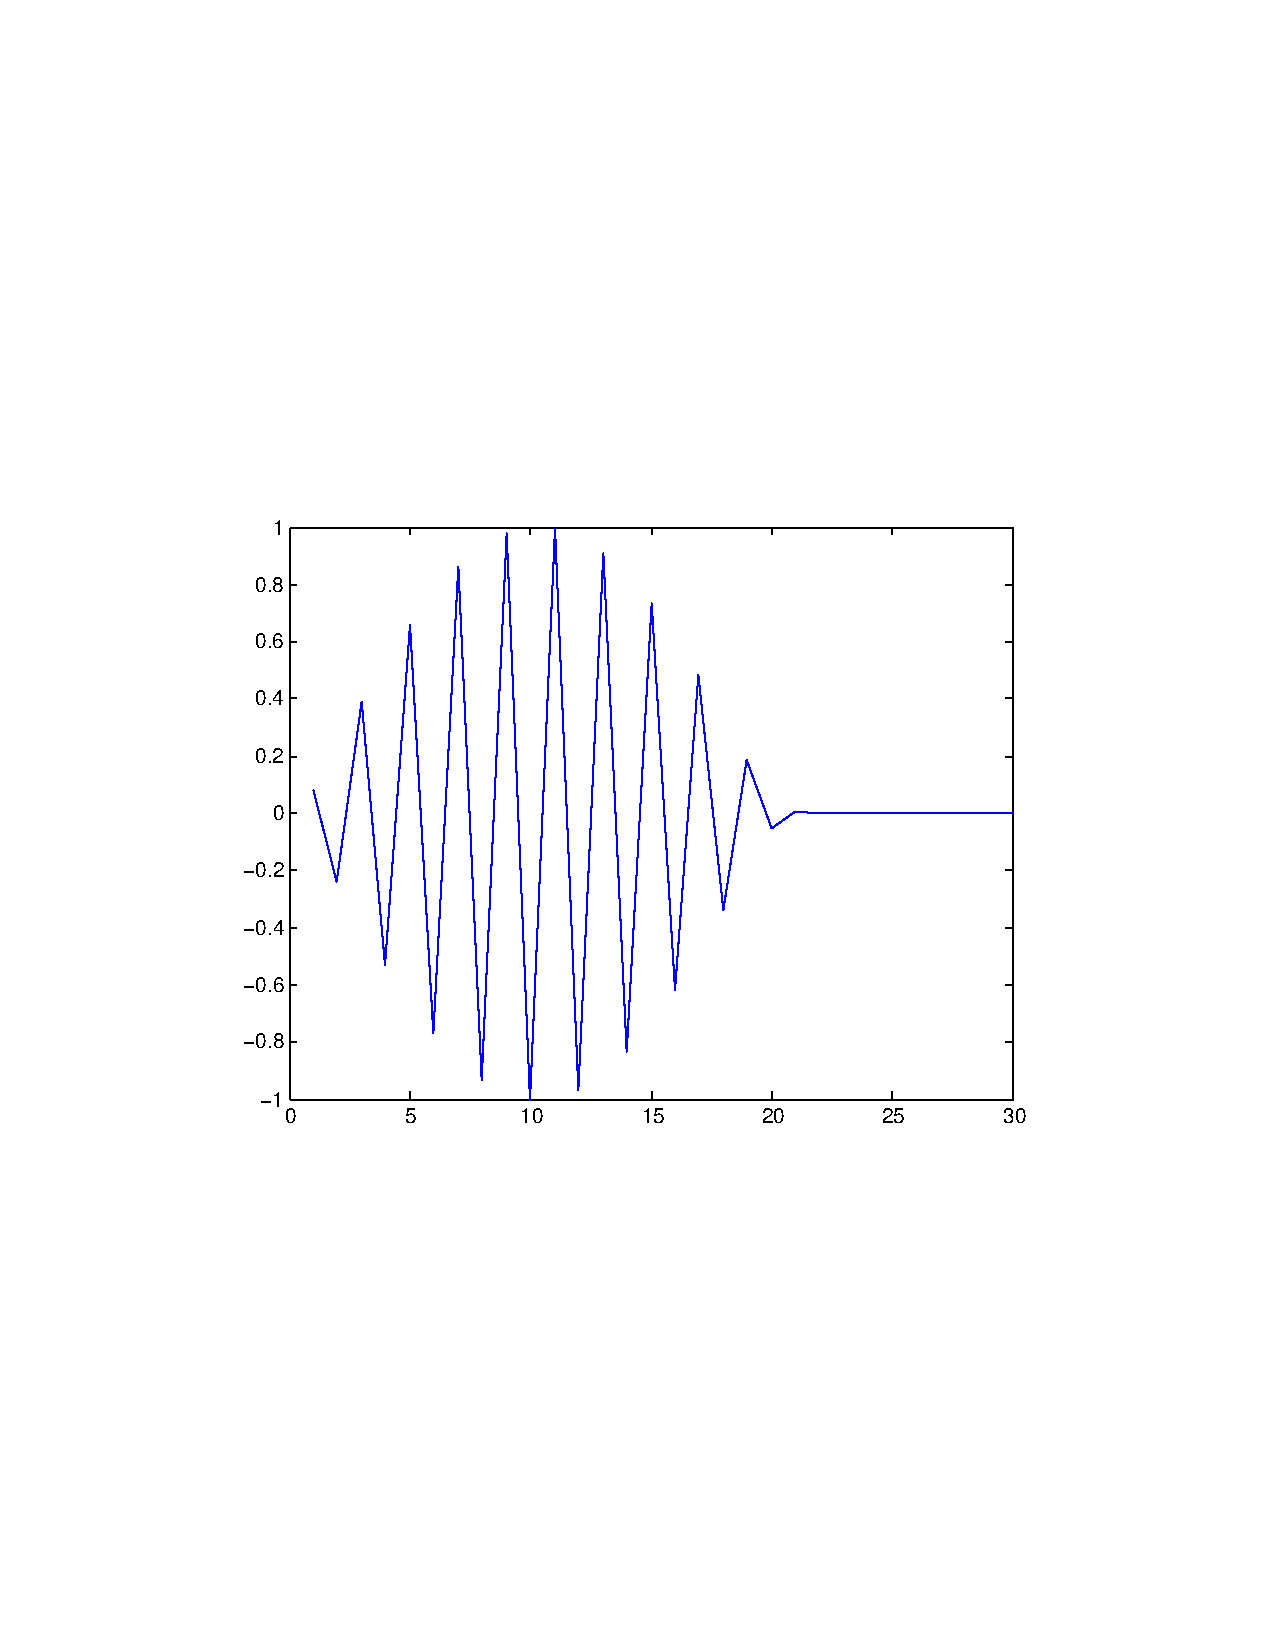
\epsfig{file=images/concentracionneutrones.pdf, width=400px}
 %      \caption[Gráfico de la concentración de neutrones]{Concentración de neutrones en estado estacionario %en función de la distancia $x$.}
 %    \label{fig:graficoNeutrones}
 % \end{center}
%\end{figure*}
%
% References
%
\bibliography{paper}

\end{document}

